\documentclass{article}
\usepackage{tikz}
\usetikzlibrary{arrows.meta}

\begin{document}
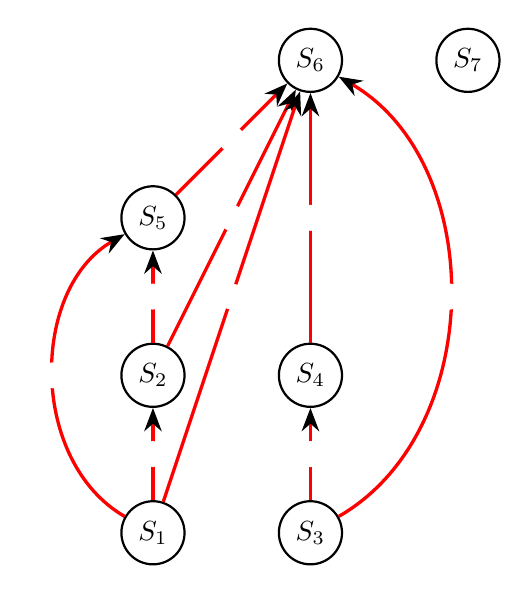
\begin{tikzpicture}
    \begin{scope}[every node/.style={circle, thick, draw}]
        \node (s1) at (4,0) {$S_1$};
        \node (s2) at (4,2) {$S_2$};
        \node (s5) at (4,4) {$S_5$};
        \node (s3) at (6,0) {$S_3$};
        \node (s4) at (6,2) {$S_4$};
        \node (s6) at (6,6) {$S_6$};
        \node (s7) at (8,6) {$S_7$};
    \end{scope}

    \begin{scope}[>={Stealth[black]}, every node/.style={fill=white, circle}, every edge/.style={draw=red, very thick}]
        \path [->] (s1) edge node {} (s2);
        \path [->] (s2) edge node {} (s5);
        \path [->] (s5) edge node {} (s6);
        \path [->] (s2) edge node {} (s6);
        \path [->] (s1) edge node {} (s6);
        \path [->] (s3) edge node {} (s4);
        \path [->] (s4) edge node {} (s6);
        \path [->] (s1) edge[bend left=60] node {} (s5);
        \path [->] (s3) edge[bend right=60] node {} (s6);
    \end{scope}
\end{tikzpicture}
\end{document}